\documentclass[12pt,a4paper]{article}

\usepackage[utf8]{inputenc}
\usepackage{amsmath}
\usepackage{amsfonts}
\usepackage{amssymb}
\usepackage{graphicx}
    
\usepackage[left=2.5cm,right=2.5cm,top=2cm,bottom=3cm]{geometry}
    
\usepackage[round]{natbib}
\usepackage{hyperref}

%%%%%%%%%%%%%%%% Code Listing %%%%%%%%%%%%%%%%%%%%%%%%%%%%%%%
\usepackage{listings}
\usepackage{color}

\definecolor{mygreen}{rgb}{0,0.6,0}
\definecolor{mygray}{rgb}{0.5,0.5,0.5}
\definecolor{mymauve}{rgb}{0.58,0,0.82}

\lstset{ %
  backgroundcolor=\color{white},   % choose the background color; you must add \usepackage{color} or \usepackage{xcolor}
  basicstyle=\footnotesize,        % the size of the fonts that are used for the code
  breakatwhitespace=false,         % sets if automatic breaks should only happen at whitespace
  breaklines=true,                 % sets automatic line breaking
  captionpos=b,                    % sets the caption-position to bottom
  commentstyle=\color{mygreen},    % comment style
  deletekeywords={...},            % if you want to delete keywords from the given language
  escapeinside={\%*}{*)},          % if you want to add LaTeX within your code
  extendedchars=true,              % lets you use non-ASCII characters; for 8-bits encodings only, does not work with UTF-8
  frame=single,                    % adds a frame around the code
  keepspaces=true,                 % keeps spaces in text, useful for keeping indentation of code (possibly needs columns=flexible)
  keywordstyle=\color{blue},       % keyword style
  language=Matlab,                 % the language of the code
  morekeywords={*,...},            % if you want to add more keywords to the set
  numbers=left,                    % where to put the line-numbers; possible values are (none, left, right)
  numbersep=5pt,                   % how far the line-numbers are from the code
  numberstyle=\tiny\color{mygray}, % the style that is used for the line-numbers
  rulecolor=\color{black},         % if not set, the frame-color may be changed on line-breaks within not-black text (e.g. comments (green here))
  showspaces=false,                % show spaces everywhere adding particular underscores; it overrides 'showstringspaces'
  showstringspaces=false,          % underline spaces within strings only
  showtabs=false,                  % show tabs within strings adding particular underscores
  stepnumber=2,                    % the step between two line-numbers. If it's 1, each line will be numbered
  stringstyle=\color{mymauve},     % string literal style
  tabsize=2                        % sets default tabsize to 2 spaces
}
%%%%%%%%%%%%%%%%%%%%%%%%%%%%%%%%%%%%%%%%%%%%%%%%%%%%%%%

\usepackage{textcomp}
\author{
  A. Theodorou\\
  \texttt{theoda@ipta.demokritos.gr}
}
\author{
  A. Theodorou\\
  \texttt{theoda@ipta.demokritos.gr}
  \and
  G. Apostolopoulos\\
  \texttt{gapost@ipta.demokritos.gr}
}
\date{June 2020}
\title{\texttt{pcpsim} \\ 
MODEL FOR HOMOGENEOUS PRECIPITATION KINETICS in \texttt{GNU OCTAVE}
}
     
\begin{document}

\maketitle

\section{Introduction}
The model for homogeneous isothermal precipitation is partly based on the model by Langer and Schwartz, as modified by Kampmann and Wagner (MLS model) and describes the nucleation and growth of  precipitates from a solid solution.


\section{Theoretical background}

\subsection{Nucleation}

As a first step we need to define the driving force for precipitation at any given time of the aging process: 
\begin{equation}
\Delta g = - \frac{kT}{V_{at}} \cdot S 
\end{equation}
with
\begin{equation}
S =  X_p \ln\frac{X}{X_{eq}} + (1 - X_p) \ln\frac{1 - X}{1-X_{eq}} 
\end{equation}
where $V_{at}$ is the atomic volume (considered as constant for all species, $V_{at}=a^3/2$ for a bcc structure with lattice parameter $a$), $S$ is a thermodynamical function giving the driving force for nucleation (based
on the hypothesis of a diluted and regular solid solution), $X_{eq}$ is the equilibrium solute mole fraction in the matrix, $X_p$ the solute mole fraction in the precipitate, and $X$ the current solute mole fraction of the matrix. The above relation has been derived by \citet{Aaronson-1970-Thevolumefreeener}.

The nucleation rate is:
\begin{equation}
\label{eq:nucleation}
J_s = \frac{d N}{d t} = Z \beta^* \exp(-\frac{\Delta G^*}{kT}) \exp(-\frac{t_i}{t})
\end{equation}
where $N$ is the number of nuclei per atomic site, $Z$ is the Zeldovich factor ($\approx$ 1/20) and $t_i$ is the incubation time. The other parameters of equation are expressed as follows:

\begin{subequations}
	\begin{align}
\beta^* &= \frac{4\pi R^{*2} D X}{a^4} \\
R^* &= \frac{2\gamma V_{at}}{S\,kT} \\
\Delta G^* &= \frac{4}{3}\pi R^{*2}\gamma \\
t_i &= \frac{1}{2\beta^* Z} 
	\end{align}	
\end{subequations}
where $R^*$ and $\Delta G^*$ are the critical nucleation radius and free energy, respectively, $\gamma$ is the matrix/precipitate interfacial energy and $D$ is the diffusion coefficient of solute atoms in the matrix.


\subsection{Growth}

A precipitate with $R>R^*$ grows by incorporating solute atoms from the surrounding matrix. Thus there is a flow of solute atoms from the matrix towards the precipitate surface. It is assumed that a steady-state is reached where there is a constant gradient of the solute concentration around the precipitate $X(r)$ that supports the solute flow $J = -D\,dX/dr |_{r=R}$, where $D$ is the diffusion constant of solute atoms in the matrix.

By solving the steady-state diffusion equation $\nabla^2 X(r)=0$ in the region around the precipitate the following equation is obtained
\begin{equation}
\frac{dR}{dt} = \frac{D}{R} \; \frac{X-X_R}{X_p-X_R}
\label{eq:growth}
\end{equation}
where $X_R$ is the solute concentration at the matrix/precipitate interface.
$X_R$ should be equal to the equilibrium concentration as modified by the Gibbs-Thomson effect (surface tension). In the \textit{ideal solution} approximation $X_R$ is given by \citep{Calderon-1994-Ostwaldripeningin}:
\begin{equation}
X_R =  X_{eq} \cdot \exp \left( \frac{2\gamma V_{at}}{kT\, R} \frac{1-X_{eq}}{X_p - X_{eq}}\right) 
\end{equation}

\subsection{Coarsening}

When the system reaches the coarsening region the average precipitate radius grows as
\begin{equation}
R^3(t) = K\cdot t
\end{equation}
where $K$ is given in the \textit{ideal solution} approximation by \citep{Calderon-1994-Ostwaldripeningin}
\begin{equation}
K\approx K_{\text{IS}} = \frac{8}{9}\frac{D \gamma V_{at}}{kT}\;
\frac{X_{eq}\, (1-X_{eq})}{(X_p - X_{eq} )^2}
\end{equation}
Thus the time differential of $R$ is given by
\begin{equation}
\frac{dR}{dt} = \frac{8}{27}\;
\frac{D \gamma V_{at}}{kT\,R^2}\;
\frac{X_{eq}\, (1-X_{eq})}{(X_p - X_{eq} )^2}
\end{equation}

\section{Nucleation \& Growth equations for the mean precipitate radius}

In many cases we may ignore the precipitate size distribution and consider only the mean radius $\bar{R}$.

In this approximation the mean radius grows according to \eqref{eq:growth} while new precipitates of radius $R^*$ nucleate at a rate given by \eqref{eq:nucleation}. Thus the mean radius evolves as 
\begin{equation}
\label{P_radius}
\frac{d\bar{R}}{dt} = \frac{D}{\bar{R}} \cdot \frac{X - X_R}{X_p - X_R} - \frac{1}{N}\frac{dN}{dt} \cdot (\bar{R} - \alpha R^*)
\end{equation}
where the 2nd term expresses the reduction rate of $\bar{R}$ due to the nucleation of new critical nuclei. $\alpha$ is a value just above 1 (e.g. 1.05) which results from the fact that new precipitates only grow if their size is slightly larger than the nucleation size.

As precipitates grow they consume solute atoms and thus the matrix concentration $X$ will be reduced from the initial $X_0$. The solute balance can be expressed as:
\begin{equation}
X_0 = X\,(1-F) + X_p\,F
\end{equation}
where $F=\frac{4}{3}\pi R^3 N$ is the precipitate volume fraction. The derivative of $X$ can be obtained from the last equation:
\begin{equation}
\frac{dX}{dt} = -(X_p - X)\, \frac{F}{1-F} \,
\left[ 3\frac{\dot{R}}{R} + \frac{\dot{N}}{N} \right]
\end{equation}  

\subsection{Dimensionless formulation}
Now the following dimensionless variables are defined that are easier to use for programming:
\begin{subequations}
	\begin{align}
t' &= \frac{D\cdot t}{r_{at}^2} \\
R' &= R / r_{at}
	\end{align}
\end{subequations}
where $r_{at} = (3V_{at}/4\pi)^{1/3}$ is the atomic radius.

The equations (\ref{eq:nucleation}), (\ref{P_radius}) plus the differential of the solute balance constitute a system of ordinary differential equations (ODEs) for $N$, $R'$ and $X$, which is rewritten here in terms of dimensionless variables:
\begin{subequations}
\label{eq:ngode}
\begin{align}
\frac{dN}{dt'} &= 
\frac{\beta_0 X}{S^2} 
\exp\left( -\frac{\Delta G_0}{S^2}\right)  
\exp\left( -\frac{S^2}{2\beta_0 X t'}\right)  \\
%%%%
\frac{dR'}{dt'} &=  
\frac{X - X_R}{X_p - X_R} 
\; \frac{1}{R'}
+ 
\frac{1}{N}\frac{dN}{dt'}
\left( \frac{\alpha R_0}{S} - R' \right) \\
\frac{dX}{dt'} &= -(X_p - X)\, \frac{F}{1-F} \,
\left[ 3\frac{\dot{R'}}{R'} + \frac{\dot{N}}{N} \right]
\end{align}
\end{subequations}
where the following definitions have been made
\begin{subequations}
\begin{align}
R_0 &= \frac{2\gamma V_{at}}{r_{at}kT} \\ 
\beta_0 &= 4\pi R_0^2 Z r_{at}^4/ a^4 \\
\Delta G_0 &= R_0^3/2  
\end{align}
\end{subequations}

Additionally the following hold
\begin{subequations}
\begin{align}
X_R &= X_{eq} \exp 
\left( \frac{R_0}{R'} \frac{1-X_{eq}}{X_p - X_{eq}}\right) \\
F &= R'^3 N
\end{align}
\end{subequations}

In the following we will omit the prime from $t'$ and $R'$.

\subsection{Implementation in \texttt{OCTAVE}}

The function file \texttt{mean\_radius/mean\_radius\_ng.m} defines the ODE system of \eqref{eq:ngode} so that it can be used in \texttt{MATLAB/OCTAVE} ODE solvers.

The content is listed below: 

\lstinputlisting{../mean_radius/mean_radius_ng.m}

\pagebreak

\subsection{Example calculation}

An example calculation using the mean radius ODEs is in \texttt{mean\_radius/FeC\_meanR\_nucl.m}. The ODEs are integrated using the solver \texttt{ode23}.

\begin{figure}[h]
\centering
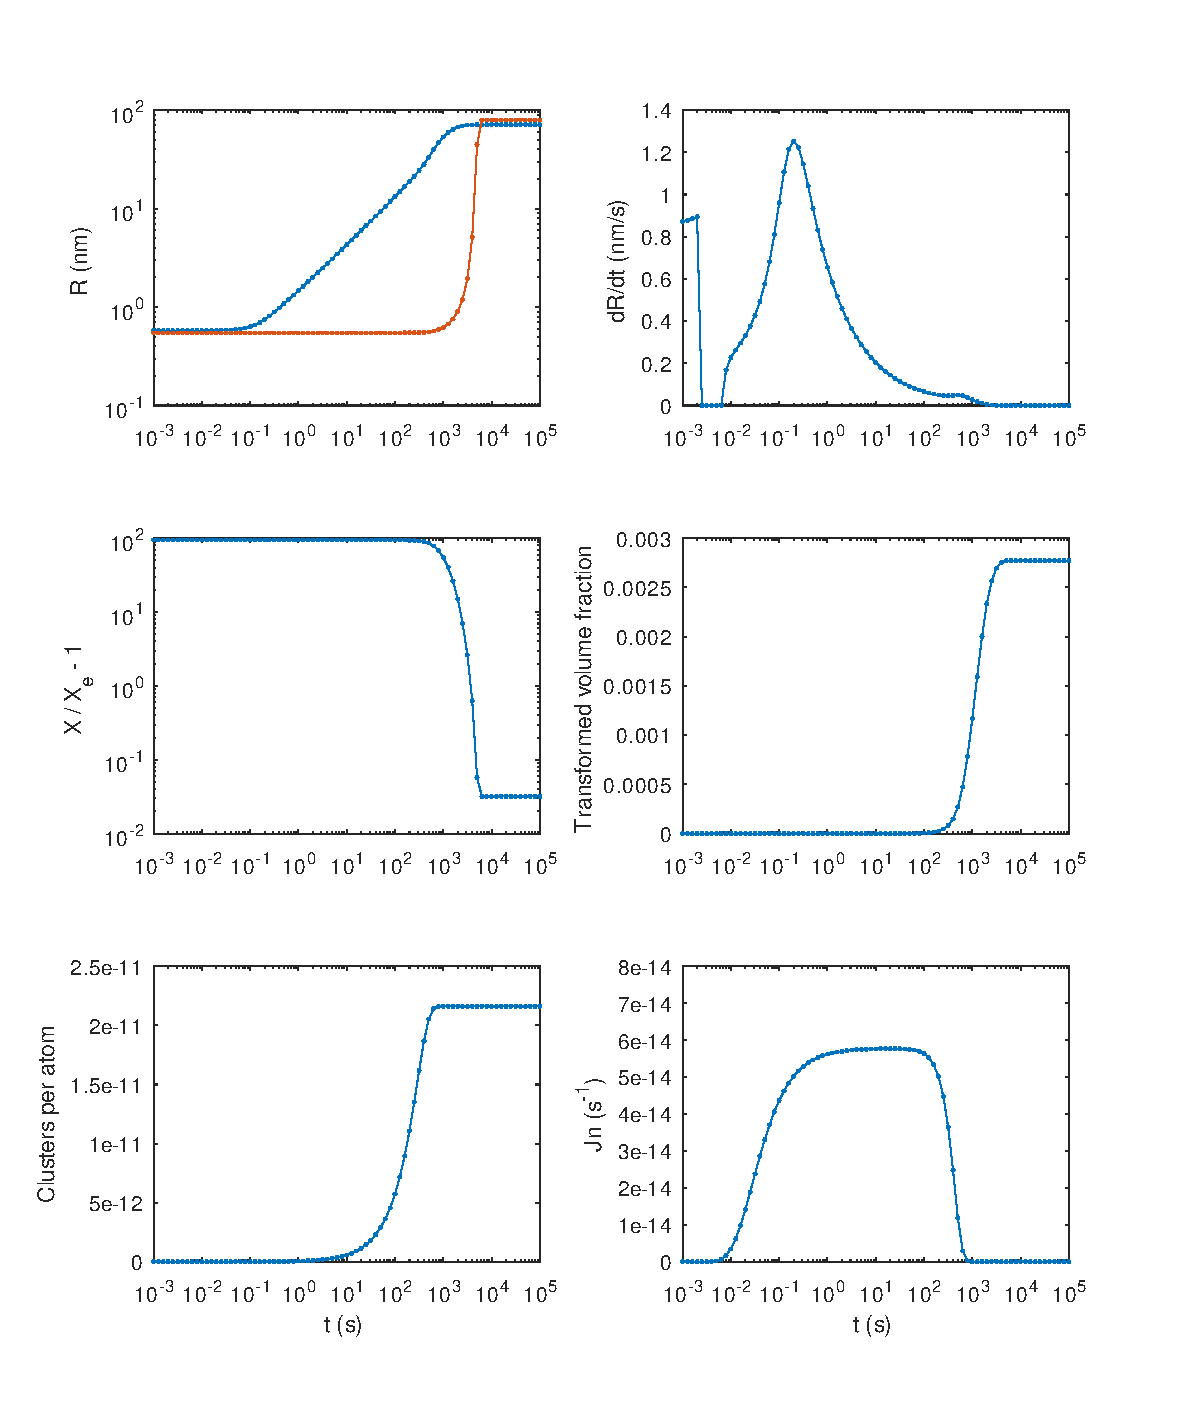
\includegraphics[width=14cm]{../mean_radius/FeC_meanR_nucl.pdf} 
\caption{Nucleation of Fe$_3$C carbide in a Fe - 0.07 at.\% C alloy at 487~K calculated with the mean radius ODEs. Model parameter: $\gamma = 0.174$~J/m$^2$. Compare to \citet{Perez-2003-ID509}}
\end{figure}

\pagebreak

\section{Numerical evolution of the precipitate size distribution (PSD)}

In this type of modelling, first discussed by Kampmann \& Wagner (see \citet{Wagner-2005-HomogeneousSecond-P}, the ``N-modell'',) we consider the evolution of the precipitate distribution function with respect to radius, $f(R,t)$. The PSD satisfies the equation of continuity:
\begin{equation}
\label{continuity}
\frac{\partial f}{\partial t} + \frac{\partial }{\partial R} (f \cdot v_R) = J_s \cdot \delta(R - \alpha R^*)
\end{equation}
where the precipitate growth rate $v_R = dR/dt$ is given by \eqref{eq:growth}. The source term on the right side of \eqref{continuity} describes the generation of new nuclei with radius $\alpha R^*$ at a rate given by $J_s$ from eq. \eqref{eq:nucleation}.

This PDE is solved numerically by discretizing the $(t,R)$ space and approximating the partial derivatives by finite differences. Defining the grid points $(t_i, R_k)$, where $(i,k)$ are integers, the discretized distribution is defined as
\begin{equation}
f_{ik} = \frac{1}{\Delta R_k} \int_{R_{k-1}}^{R_k}f(R,t_i)\,dR
\end{equation}
and the discretized PDE becomes
\begin{equation}
\label{PDE}
\frac{f_{i+1,k} - f_{ik}}{\Delta t_i} = - \frac{J_{ik} - J_{i,k-1}}{\Delta R_k} + \frac{J_s}{\Delta R_{k^*+1}} \delta_{k,k^*+1}
\end{equation}
where the precipitate ``current'' $J_{ik}$ is given by
\begin{equation} 
J_{ik} = 
\begin{cases}
f_{ik}v_k & v_k \geq 0 \\
f_{i,k+1}v_k & v_k<0
\end{cases}
\end{equation}
The above finite difference scheme has been introduced by \citet{Myhr-2000-Modellingofnon-iso} for this type of calculation and corresponds to ``\textit{upwind differencing}'' used in CFD (see Press et al. ``Numerical Recipes'', ch. 20).

The index $k^*$ corresponds to the spatial grid point where $R_{k^*-1} \leq  R^* < R_{k^*}$. The generated nuclei are added to $f_{i,k^*+1}$ so that all of them survive and grow. \footnote{If the generated nuclei where added to $f_{i,k^*}$ a fraction of them would dissolve since $v_{k^*-1}<0.$ }

The total precipitate concentration, average radius and volume fraction can be obtained from $f_{i,k}$ by the following relations:
\begin{subequations}
	\begin{align}
N_i &= \int_0^\infty f(R,t_i) dR 
\approx \sum_k { f_{i,k} \Delta R_k } \\
\bar{R}_i &= \frac{1}{N_i}\int_0^\infty f(R,t_i) R dR
\approx \frac{1}{2 N_i}\sum_k { f_{i,k} (R_k^2-R_{k-1}^2 ) }  \\
F_i &= \frac{4\pi}{3V_{at}} \int_0^\infty f(R,t_i) R^3 dR
\approx \frac{1}{4\, r_{at}^3} \sum_k { f_{i,k} (R_k^4-R_{k-1}^4 )  } 
	\end{align}
\end{subequations}

\subsection{Numerical integration}

A static logarithmic grid is selected for the $R$-space discretization with constant $\Delta R_k / R_k$ (typically $\sim 0.05$.) The first point is typically positioned just below $R^*$ and the last point should be higher than the largest anticipated radius $R_{\max}$ for the simulation period. To obtain an estimate of $R_{\max}$ we define the function $\tau(R)$
\[
\tau(R) = \int_{R^*}^{R}{\frac{dR}{v_R}}
\] 
where the initial solute concentration $X_0$ is employed in the evaluation of $v_R$. This function corresponds to the time needed for a precipitate to grow to radius $R$. Then $R_{\max}$ is found by solving numerically the equation $\tau(R_{\max}) = t_s$, where $t_s$ the total simulation time.

The PSD is initialized either to zero or to some initial precipitation state obtained either from experiment or other simulation.

The evolution of the PSD is done iteratively with the following steps:
\begin{enumerate}
\item Calculate the current volume fraction $F_i$ and matrix concentration $X$
\item Calculate the nucleation rate $J_s$ and the bin index $k^*$ where the generated nuclei are to be inserted.
\item Calculate the right side of eq. \eqref{PDE}.
\item Adaptively decide the time step $\Delta t_i$ (see below)
\item Advance the PSD to $f_{i+1,k}$ and simulation time
\item Repeat until the total simulation time is reached 
\end{enumerate}

\subsubsection{Adaptive time step selection}
$\Delta t_i$ is selected according to 2 criteria.

First, an upper limit is set by the following relation
\begin{equation}
v_k  \Delta t_i < \Delta R_k, \quad \forall k
\end{equation}
This is the well-known \textit{Courant condition} which ensures the stability of the PDE numerical solution (again see Press et al. ``Numerical Recipes'', ch. 20). Essentially it means that in one time-step nuclei from one distribution bin can move only to adjacent bins and not further away. Thus the time interval is initially set by
\begin{equation}
\Delta t_i = \min \left\lbrace  | \Delta R_k / v_k | \right\rbrace 
\end{equation}

A second criterion is set by the requirement that $R^*$, which is a critical simulation parameter, does not change appreciably during a time step. Typically we require that $\Delta R^* / R^* < 0.01$. To implement this, $f_{i+1,k}$ and the new $R^*$ must first be calculated with the current value of $\Delta t_i$; if the change of $R^*$ is too large the time step is halved and $f_{i+1,k}$ is recalculated. The process is repeated until the criterion is fulfilled. 

\subsubsection{Lower cut-off radius} 

A drawback of the method is that the time step is bounded by the smallest $\Delta R_k / v_k$ which occurs at the lower $R$ bins. However, as the simulation advances and the average radius becomes larger, the concentration in the first few bins becomes very low and can be neglected. Thus we define a lower cut-off index $k_c$ and set $f=0$ for $R<R_{k_c}$. The grid points below $k_c$ are not considered when selecting  $\Delta t_i$ and this allows for much more efficient simulation in the growth phase. 

The cut-off index $k_c$ is initially set to the 1st grid point and then it is advanced by one each time the concentration in the 1st bin above cut-off, $f_{i,k_c+1}\cdot \Delta R_{k_c+1}$, falls below a certain threshold $N_{min}$. A reasonable threshold could be 1 nucleus per cm$^3$ or, equivalently, $N_{min}\sim 10^{-23}$. This means that effectively when the concentration in the first bin above $k_c$ falls below $N_{min}$, the bin is zeroed-out and becomes inactive. 

When nuclei dissolution occurs the distribution will move gradually towards smaller $R$ and we have to allow $k_c$ to go down again, i.e., to gradually reactivate the lower bins of the distribution. For this we check the concentration $\delta N_c$ of nuclei that would move from bin $k_c+1$ towards $k_c$ during a time-step. This is equal to 
\[
\delta N_c = |v_{k_c}| f_{i,k_c+1} \Delta t_i
\] 
If $\delta N_c$ becomes larger than a threshold then the cut-off index $k_c$ is decreased by one. This threshold is selected as
\begin{equation}
\delta N_c \geq N_{min} + \epsilon N
\end{equation}
where $N = \sum_k {f_{i,k} \Delta R_k}$ is the total concentration of nuclei and $\epsilon$ a small number (typically $10^{-3}$ or $10^{-4}$). Here the relative term $\epsilon N$ is used to raise the threshold, otherwise the lower cut-off will extend to very small $R$ and the simulation will become significantly slower. 

\bibliographystyle{plainnat}
\bibliography{pcpsim}

\end{document}
 